\section{Discussion} \label{sec:discussion}

To the best of our knowledge, this is the first research work that investigates
the sustainability of academic software regarding its publicization, evolution
stage in the life cycle, and recognition. 
We performed three exploratory studies in the domain of
academic software for static analysis, based on software publications from ASE
and SCAM, two relevant software engineering conferences. ASE is more general in
scope and SCAM is concerned with source code analysis.

\paragraph{\bf Evolution of the recognition of academic software for static
analysis published in ASE and SCAM} The academic software has received more
attention in the academic literature over time; there is a clear
growth in the total number of references to software for static analysis in
publications of the ACM and IEEE databases, as Figure~\ref{mentions-by-year}
shows.

\begin{figure}[ht]
  \centering
  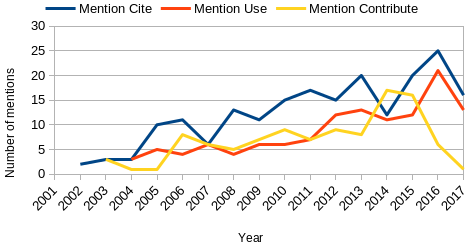
\includegraphics[scale=0.59]{figs/mentions-type-by-year.png}
  \caption{Total number of mentions per type and year.}
  \label{mentions-by-year}
\end{figure}

This growth, however, may be influenced by the increase in the number of
projects each year. By isolating the data and keeping the number of projects
constant over time, there is a growth of 38\% per year, according to
Figure~\ref{mentions-trend}.

\begin{figure}[ht]
  \center
  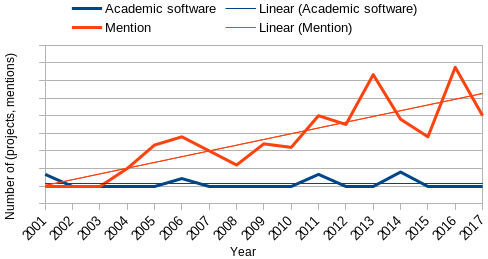
\includegraphics[scale=0.59]{figs/mentions-trend.png}
  \caption{Growth in the number of mentions per year.}
  \label{mentions-trend}
\end{figure}

Among the 60 academic software projects of static analysis studied, 13 projects
(22\%) did not have academic recognition, i.e., they were mentioned only in
the original article published in ASE or SCAM, where the software was introduced. The
other 47 projects (78\%) had greater academic recognition, whereas mentions
have been found in one or more articles other than the first publication.

\paragraph{\bf Influence of the life cycle stage on the recognition of academic
software} There were 160 mentions for projects in close-down stage.
This data
possibly indicates that papers published before the project enter this stage or
indicating that the project is accessible only to its authors but not for the
general public.
%
For other life cycle stages, we found 71 mentions for projects
in evolution or servicing stages and 131 mentions for projects in the initial
development stage.

We found a large number of mentions for ESBMC, PARSEWeb,
and TestEra, including recent publications
between 2016 and 2017; however, the fact that they are in the close-down stage
demands attention, since they are not publicly available but continue to
receive attention from academia.
